\documentclass [a4paper] {article}

\usepackage[utf8]{inputenc}


\title{\textbf{Practica 1: Fundamentos de la ciencia de datos}}
\author{Luis Alejandro Cabanillas, Alvaro de las Heras, Mohssin Nagib Najim}

\usepackage{Sweave}
\begin{document}

\maketitle

\section{Ejercicio 1} En la primera parte se realizará un ejercicio de prueba con distintos tipos de ficheros para probar la 
carga de datos en R. Una vez tengamos estos datos se procederá con su análisis. 

\subsection{Lectura y operaciones sobre .txt} 
Lo primero que vamos a hacer es la carga del fichero .txt en R. Este tipo de archivo es soportado directamente
por R sin necesidad de bibliotecas externas, al igual que el CSV. El archivo que se va a cargar contiene
los nombres de satélites del planeta Urano junto a sus radios. 
Para la carga del fichero utilizaremos la instrucción read.table("archivo.txt"). Tenemos que tener en cuenta que 
el archivo tiene que estar en el directorio actual de trabajo, sino deberemos introducir la ruta hasta el mismo.
Algunas instrucciones útiles relacionadas con el directorio de trabajo en R son:

\begin{itemize}
	\item \textbf{getwd()}: Nos proporciona el directorio de trabajo actual. 
	\item \textbf{setwd("directorio")}: Cambia el directorio de trabajo actual al directorio 
											especificado.
	\item \textbf{list.files()}: Muestra una lista de los archivos del directorio actual de trabajo.
														 
\end{itemize}

Asi, lo primero que tenemos que hacer es comprobar que el archivo satelites.txt se encuentra en el directorio de trabajo actual:
\begin{Schunk}
\begin{Sinput}
> getwd()
\end{Sinput}
\begin{Soutput}
[1] "C:/Users/Cliri/Desktop/2.p1"
\end{Soutput}
\begin{Sinput}
> list.files()
\end{Sinput}
\begin{Soutput}
 [1] "cardata.sav"       "ej2.R"             "Fifa"             
 [4] "Practica1-030.pdf" "Practica1-031.pdf" "Practica1-034.pdf"
 [7] "Practica1-041.pdf" "Practica1.aux"     "Practica1.log"    
[10] "Practica1.pdf"     "Practica1.Rnw"     "Practica1.tex"    
[13] "rango.R"           "satelites.csv"     "satelites.txt"    
\end{Soutput}
\begin{Sinput}
> 
\end{Sinput}
\end{Schunk}
Como podemos ver, el archivo se encuentra en el directorio especificado, por lo que podemos hacer uso de read.table() para la carga de datos del fichero:
\begin{Schunk}
\begin{Sinput}
> satelites<-read.table("satelites.txt")
> satelites
\end{Sinput}
\begin{Soutput}
       satelite radio
1      Cordelia    13
2        Ofelia    16
3        Bianca    22
4       Cresida    33
5     Desdemona    29
6       Julieta    42
7     Rosalinda    27
8       Belinda    34
9  Luna-1986U10    20
10     Calibano    30
11   Luna-199U1    20
12   Luna-199U2    15
\end{Soutput}
\end{Schunk}

Una vez que tenemos todos los datos cargados en R, procedemos a su análisis.

\subsubsection{Calculo del rango}
Para facilitar los cálculos, vamos a almacenar en una variable radio todos los radios de los satélites de Urano mediante el símbolo del dolar,  
que nos permite extraer subconjuntos en R:

\begin{Schunk}
\begin{Sinput}
> radio=satelites$radio
> radio
\end{Sinput}
\begin{Soutput}
 [1] 13 16 22 33 29 42 27 34 20 30 20 15
\end{Soutput}
\begin{Sinput}
> 
\end{Sinput}
\end{Schunk}
En R no tenemos ninguna funcion específica para calcular el rango, por lo que la emplearemos nosotros. Para ello, haremos uso de:
\begin{itemize}
	\item \textbf{max()}: Nos devuelve el valor máximo de uno o varios vectores.
	\item \textbf{min()}: Nos devuelve el valor mínimo de uno o varios vectores. 
																									 
\end{itemize}

De esta forma creamos la funcion rango y la aplicamos a nuestro problema:
\begin{Schunk}
\begin{Sinput}
> rango = function(radio){max(radio)-min(radio)}
> rang = rango(radio)
> 
\end{Sinput}
\end{Schunk}

El rango obtenido es 29

Para guardar la función rango creada haremos uso de dos funciones de R:
\begin{itemize}
	\item \textbf{dump("nombre funcion","nombre archivo")}: Crea y guarda en un archivo la función especificada.
	\item \textbf{source("nombre archivo")}: Lee el archivo .R que le pasemos.
																									 
\end{itemize}

De esta forma:
\begin{Schunk}
\begin{Sinput}
> dump("rango", file="rango.R")
> source("rango.R")
> 
\end{Sinput}
\end{Schunk}

\subsubsection{Cálculo de frecuencias}
\paragraph{Frecuencia absoluta}
Para el cálculo de la frecuencia absoluta haremos uso de la función \textbf{table("vector")} de R, que
creará una tabla en la que aparecerá cuantas veces aparece cada radio:
\begin{Schunk}
\begin{Sinput}
> frecabsradio <- table(radio)
> frecabsradio
\end{Sinput}
\begin{Soutput}
radio
13 15 16 20 22 27 29 30 33 34 42 
 1  1  1  2  1  1  1  1  1  1  1 
\end{Soutput}
\begin{Sinput}
> 
\end{Sinput}
\end{Schunk}
Vemos que todos los radios aparecen una vez, salvo el 20 que aparece dos veces.

\paragraph{Frecuencia absoluta acumulada.}
El cálculo de la frecuencia absoluta acumulada será muy sencillo, ya que lo único que tenemos que
hacer es llamar a la función \textbf{cumsum("vector")} de R, que irá calculando la suma acumulada
de las frecuencias absolutas calculadas anteriormente.
\begin{Schunk}
\begin{Sinput}
> frecabsacumradio <- cumsum(frecabsradio)
> frecabsacumradio
\end{Sinput}
\begin{Soutput}
13 15 16 20 22 27 29 30 33 34 42 
 1  2  3  5  6  7  8  9 10 11 12 
\end{Soutput}
\end{Schunk}

\paragraph{Frecuencia relativa.}
En R no tenemos una funcion que nos calcule las frecuencias relativas, asi que tendremos que crearla
nosotros haciendo uso de la fórmula:
\begin{Schunk}
\begin{Sinput}
> frecrel = function(radio){table(radio)/length(radio)}
> frecrel(radio)
\end{Sinput}
\begin{Soutput}
radio
        13         15         16         20         22         27         29 
0.08333333 0.08333333 0.08333333 0.16666667 0.08333333 0.08333333 0.08333333 
        30         33         34         42 
0.08333333 0.08333333 0.08333333 0.08333333 
\end{Soutput}
\end{Schunk}

Como el radio=20 es el único que aparece dos veces, su frecuencia relativa es diferente a la del resto.

\paragraph{Frecuencia relativa acumulada.}
Para el cálculo de la frecuencia relativa acumulada únicamente tendremos que hacer una suma acumulada de
las frecuencias relativas obtenidas en el apartado anterior:
\begin{Schunk}
\begin{Sinput}
> frecrelacumradio <- cumsum(frecrel(radio))
> frecrelacumradio
\end{Sinput}
\begin{Soutput}
        13         15         16         20         22         27         29 
0.08333333 0.16666667 0.25000000 0.41666667 0.50000000 0.58333333 0.66666667 
        30         33         34         42 
0.75000000 0.83333333 0.91666667 1.00000000 
\end{Soutput}
\end{Schunk}

\subsubsection{Cálculo de la media aritmética}
Para el cálculo de la media aritmética en R tenemos la función \textbf{mean("vector")}, que
nos devuelve la media aritmética de una serie de valores almacenados en un vector. Así:
\begin{Schunk}
\begin{Sinput}
> media<-mean(radio)
> media
\end{Sinput}
\begin{Soutput}
[1] 25.08333
\end{Soutput}
\end{Schunk}

La media obtenida es 25.0833333333333

\subsubsection{Medidas de dispersion}
\paragraph{Desviacion tipica.}
R nos proporciona \textbf{sd("vector")} para el cálculo de la desviación típica:
\begin{Schunk}
\begin{Sinput}
> desTip<-sd(radio)
> desTip
\end{Sinput}
\begin{Soutput}
[1] 8.857029
\end{Soutput}
\end{Schunk}
La desviación típica obtenida es 8.8570293946091
\paragraph{Varianza.}
Para la varianza también tenemos una formula específica en R, \textbf{var("vector")}.
\begin{Schunk}
\begin{Sinput}
> var<-var(radio)
> var
\end{Sinput}
\begin{Soutput}
[1] 78.44697
\end{Soutput}
\end{Schunk}
La varianza obtenida es 78.4469696969697

\subsubsection{Medidas de ordenacion}
\paragraph{Mediana.}
La función que nos hace la mediana en R es \textbf{median("vector")}.
\begin{Schunk}
\begin{Sinput}
> med<-median(radio)
> med
\end{Sinput}
\begin{Soutput}
[1] 24.5
\end{Soutput}
\end{Schunk}
La mediana obtenida es 24.5

\paragraph{Cuartiles.}
De nuevo, tenemos una función en R que nos calcula los cuartiles: \textbf{quantile("vector")}.
\begin{Schunk}
\begin{Sinput}
> cuart<-quantile(radio)
> cuart
\end{Sinput}
\begin{Soutput}
   0%   25%   50%   75%  100% 
13.00 19.00 24.50 30.75 42.00 
\end{Soutput}
\end{Schunk}
Los cuartiles obtenidos son 13, 19, 24.5, 30.75, 42

\paragraph{Cuantil 54.}
Para calcular el cuantil 54 lo único que tenemos que hacer es pasarle un argumento más a la función
quantile, indicándole el cuantil que queremos:
\begin{Schunk}
\begin{Sinput}
> cuart54<-quantile(radio,0.54)
> cuart54
\end{Sinput}
\begin{Soutput}
 54% 
26.7 
\end{Soutput}
\end{Schunk}
El cuartil 54 obtenido es 26.7


\subsection{Lectura y operaciones sobre .sav} 
En este apartado realizaremos el análisis sobre un tipo de fichero .sav, para cargarlo en R tendremos
que utilizar una biblioteca externa pero disponible para su inclusión fácilmente. El archivo .sav contiene datos
de automóviles, como su consumo en mpg (millas por galón), cilindrada, aceleración, etc. Para la carga de este
fichero primero debemos importar la biblioteca foreign con la instrucción \textbf{library(foreign)}, para posteriormente
poder leer el archivo .sav con la instrucción \textbf{read.spss("archivo.sav")}. 

Realizamos la carga de datos con el archivo .sav en nuestro directorio actual, como solo se nos pide analizar el dato de mpg mostraremos solo ese dato:
\begin{Schunk}
\begin{Sinput}
> library(foreign)
> autos<-read.spss("cardata.sav")
> mpg = autos$mpg
> mpg
\end{Sinput}
\begin{Soutput}
  [1] 36.1 19.9 19.4 20.2 19.2 20.5 20.2 25.1 20.5 19.4 20.6 20.8 18.6 18.1 19.2
 [16] 17.7 18.1 17.5 30.0 30.9 23.2 23.8 21.5 19.8 22.3 20.2 20.6 17.0 17.6 16.5
 [31] 18.2 16.9 15.5 19.2 18.5 35.7 27.4 23.0 23.9 34.2 34.5 28.4 28.8 26.8 33.5
 [46] 32.1 28.0 26.4 24.3 19.1 27.9 23.6 27.2 26.6 25.8 23.5 30.0 39.0 34.7 34.4
 [61] 29.9 22.4 26.6 20.2 17.6 28.0 27.0 34.0 31.0 29.0 27.0 24.0 23.0 38.0 36.0
 [76] 25.0 38.0 26.0 22.0 36.0 27.0 27.0 32.0 28.0 31.0 43.1 20.3 17.0 21.6 16.2
 [91] 31.5 31.9 25.4 27.2 37.3 41.5 34.3 44.3 43.4 36.4 30.4 40.9 29.8 35.0 33.0
[106] 34.5 28.1   NA 30.7 36.0 44.0 32.8 39.4 36.1 27.5 27.2 21.1 23.9 29.5 34.1
[121] 31.8 38.1 37.2 29.8 31.3 37.0 32.2 46.6 40.8 44.6 33.8 32.7 23.7 32.4 39.1
[136] 35.1 32.3 37.0 37.7 34.1 33.7 32.4 32.9 31.6 25.4 24.2 37.0 31.0 36.0 36.0
[151] 34.0 38.0 32.0 38.0 32.0
\end{Soutput}
\end{Schunk}

\subsubsection{Calculo del rango}
Para facilitar los cálculos, vamos a almacenar en una variable radio todos los radios de los satélites de Urano mediante el símbolo del dolar,  
que nos permite extraer subconjuntos en R, para poder realizar esta operación tenemos que eliminar todos los datos NA que contiene la variable mpg,
esto lo haremos con la función \textbf{na.omit("vector")} que nos devolverá los datos sin los NA para poder operar el rango:

\begin{Schunk}
\begin{Sinput}
> nmpg <- na.omit(mpg)
> rangmpg <- rango(nmpg)
> rangmpg
\end{Sinput}
\begin{Soutput}
[1] 31.1
\end{Soutput}
\end{Schunk}

El rango obtenido es 31.1

\subsubsection{Calculo de la media aritmética}
Para el cálculo de la media aritmetica en R utilizaremos la función \textbf{mean("vector")} como hicimos previamente que nos devolverá la media aritmética de
una serie de valores almacenados en un vector, realizamos la misma operación con los valores NA del vector:
\begin{Schunk}
\begin{Sinput}
> mediampg <- mean(nmpg)
> mediampg
\end{Sinput}
\begin{Soutput}
[1] 28.79351
\end{Soutput}
\end{Schunk}

La media obtenida es 28.7935064935065


\subsubsection{Medidas de dispersión}
\paragraph{Desviación típica.}
R nos proporciona \textbf{sd("vector")} para el cálculo de la desviación típica:
\begin{Schunk}
\begin{Sinput}
> desTipmpg<-sd(nmpg)
> desTipmpg
\end{Sinput}
\begin{Soutput}
[1] 7.37721
\end{Soutput}
\end{Schunk}
La desviación típica obtenida es 7.37720987451471
\paragraph{Varianza.}
Para la varianza también tenemos una fórmula específica en R, \textbf{var("vector")}.
\begin{Schunk}
\begin{Sinput}
> varmpg<-var(nmpg)
> varmpg
\end{Sinput}
\begin{Soutput}
[1] 54.42323
\end{Soutput}
\end{Schunk}
La varianza obtenida es 54.4232255326373

\subsubsection{Medidas de ordenación}
\paragraph{Mediana.}
La función que nos hace la mediana en R es \textbf{median("vector")}.
\begin{Schunk}
\begin{Sinput}
> medmpg<-median(nmpg)
> medmpg
\end{Sinput}
\begin{Soutput}
[1] 28.9
\end{Soutput}
\end{Schunk}

La mediana obtenida es 28.9

\paragraph{Cuartiles.}
De nuevo, tenemos una función en R que nos calcula los cuartiles: \textbf{quantile("vector")}.
\begin{Schunk}
\begin{Sinput}
> cuartmpg<-quantile(nmpg)
> cuartmpg
\end{Sinput}
\begin{Soutput}
    0%    25%    50%    75%   100% 
15.500 22.550 28.900 34.275 46.600 
\end{Soutput}
\end{Schunk}

Los cuartiles obtenidos son 15.5, 22.55, 28.9, 34.275, 46.6

\section{Ejercicio 2}
En este ejercicio se realizará un análisis a partir de un dataset de jugadores de fútbol del videojuego FIFA 19.

\subsection{Lectura del dataset}
El dataset sobre los jugadores ha sido obtenido en Kaggle, estando por defecto en formato CSV, teniendo un total de 91 columnas y 18206 filas. Sin embargo, para dar más juego
al ejercicio hemos convertido los datos a otros formatos muy utilizados como son JSON y Excel. Las conversiones las hemos hecho con el propio 
Excel y con un conversor on-line de CSV a JSON.

\subsubsection{Archivo CSV con filtro en la lectura}
La forma más sencilla de obtener los datos es leyendo el CSV, al estar integrada en el propio R.
Además se ha realizado un filtro de columnas en la lectura mediante el parámetro colClasses, poniendo el tipo deseado para las que nos interesan 
y dejando a NULL las que no, de esta forma
se consigue una lectura del archivo mucho más rápida. Otros parámetros que también se han usado han sido nrows para filtrar filas y encoding 
para poner los datos en UTF8.

\begin{Schunk}
\begin{Sinput}
> filas <- 6000
> # Lectura del CSV
> columnas<-c("NULL","NULL","character","numeric","NULL","character","NULL","numeric",
+ "numeric","character","NULL","character","character",rep("NULL",76))
> csv <- read.csv("Fifa\\fifa19.csv",head=T,sep=",",
+ encoding = "UTF-8",colClasses=columnas,nrows=filas)
> head(csv,10)
\end{Sinput}
\begin{Soutput}
                Name Age Nationality Overall Potential                Club
1           L. Messi  31   Argentina      94        94        FC Barcelona
2  Cristiano Ronaldo  33    Portugal      94        94            Juventus
3          Neymar Jr  26      Brazil      92        93 Paris Saint-Germain
4             De Gea  27       Spain      91        93   Manchester United
5       K. De Bruyne  27     Belgium      91        92     Manchester City
6          E. Hazard  27     Belgium      91        91             Chelsea
7          L. Modric  32     Croatia      91        91         Real Madrid
8          L. Suárez  31     Uruguay      91        91        FC Barcelona
9       Sergio Ramos  32       Spain      91        91         Real Madrid
10          J. Oblak  25    Slovenia      90        93     Atlético Madrid
     Value  Wage
1  \200110.5M \200565K
2     \20077M \200405K
3  \200118.5M \200290K
4     \20072M \200260K
5    \200102M \200355K
6     \20093M \200340K
7     \20067M \200420K
8     \20080M \200455K
9     \20051M \200380K
10    \20068M  \20094K
\end{Soutput}
\end{Schunk}

\subsubsection{Archivo JSON}
Para la lectura del archivo JSON se ha usado la función read json que ofrece jsonlite, aunque en un principio se hizo con rjson se descarto por su baja eficiencia. 
A diferencia del CSV, aquí no se pueden quitar columnas en la lectura sino que ha de ser sobre 
el conjunto de datos ya cargados, haciendolo más lento que el primero. Con el parámetro simplify = simplifyVector 
conseguimos que el resultado sea un data.frame de R, con el que trabajar más fácilmente. 

\begin{Schunk}
\begin{Sinput}
> install.packages("jsonlite")
\end{Sinput}
\begin{Soutput}
--- Please select a CRAN mirror for use in this session ---
package ‘jsonlite’ successfully unpacked and MD5 sums checked

The downloaded binary packages are in
	C:\Users\Cliri\AppData\Local\Temp\Rtmp2ZckqC\downloaded_packages
\end{Soutput}
\begin{Sinput}
> library("jsonlite")
> json<-read_json("Fifa\\fifa19.json", simplifyVector=TRUE)
> json<- json[-((6001):19000), -c(1,2,5,7,11,14:89)]
> head(json,10)
\end{Sinput}
\begin{Soutput}
                Name Age Nationality Overall Potential                Club
1           L. Messi  31   Argentina      94        94        FC Barcelona
2  Cristiano Ronaldo  33    Portugal      94        94            Juventus
3          Neymar Jr  26      Brazil      92        93 Paris Saint-Germain
4             De Gea  27       Spain      91        93   Manchester United
5       K. De Bruyne  27     Belgium      91        92     Manchester City
6          E. Hazard  27     Belgium      91        91             Chelsea
7          L. Modric  32     Croatia      91        91         Real Madrid
8          L. Suárez  31     Uruguay      91        91        FC Barcelona
9       Sergio Ramos  32       Spain      91        91         Real Madrid
10          J. Oblak  25    Slovenia      90        93     Atlético Madrid
     Value  Wage
1  \200110.5M \200565K
2     \20077M \200405K
3  \200118.5M \200290K
4     \20072M \200260K
5    \200102M \200355K
6     \20093M \200340K
7     \20067M \200420K
8     \20080M \200455K
9     \20051M \200380K
10    \20068M  \20094K
\end{Soutput}
\end{Schunk}

\subsubsection{Archivo Excel}
La lectura del Excel se realiza con la biblioteca readxl de CRAN. Para ello se usa el método read excel, este permite la lectura tanto de formatos xls como de xlsx. 
Como en el caso anterior las columnas no se pueden filtrar en la lectura, por lo que ha de hacerse después. Sin embargo, si permite limitar las filas 
con el parámetro n max.

\begin{Schunk}
\begin{Sinput}
> install.packages("readxl")
\end{Sinput}
\begin{Soutput}
package ‘readxl’ successfully unpacked and MD5 sums checked

The downloaded binary packages are in
	C:\Users\Cliri\AppData\Local\Temp\Rtmp2ZckqC\downloaded_packages
\end{Soutput}
\begin{Sinput}
> library("readxl")
> excel <- read_excel("Fifa\\fifa19.xlsx", n_max=6000)
> excel<- excel[, -c(1,2,5,7,11,14:89)]
> head(excel,10)
\end{Sinput}
\begin{Soutput}
# A tibble: 10 x 8
   Name            Age Nationality Overall Potential Club           Value  Wage 
   <chr>         <dbl> <chr>         <dbl>     <dbl> <chr>          <chr>  <chr>
 1 L. Messi         31 Argentina        94        94 FC Barcelona   €110.~ €565K
 2 Cristiano Ro~    33 Portugal         94        94 Juventus       €77M   €405K
 3 Neymar Jr        26 Brazil           92        93 Paris Saint-G~ €118.~ €290K
 4 De Gea           27 Spain            91        93 Manchester Un~ €72M   €260K
 5 K. De Bruyne     27 Belgium          91        92 Manchester Ci~ €102M  €355K
 6 E. Hazard        27 Belgium          91        91 Chelsea        €93M   €340K
 7 L. Modric        32 Croatia          91        91 Real Madrid    €67M   €420K
 8 L. Suárez        31 Uruguay          91        91 FC Barcelona   €80M   €455K
 9 Sergio Ramos     32 Spain            91        91 Real Madrid    €51M   €380K
10 J. Oblak         25 Slovenia         90        93 Atlético Madr~ €68M   €94K 
\end{Soutput}
\end{Schunk}

Una vez visto el proceso de carga de datos, cualquiera de los que hemos cargado servirán para realizar el análisis.

\begin{Schunk}
\begin{Sinput}
> edades <- excel$Age
> equipos <- json$Club
> nacionalidades <-csv$Nationality
> puntuaciones <- csv$Overall
\end{Sinput}
\end{Schunk}

\subsection{Frecuencias de los datos}
En el primer análisis de datos que vamos a realizar veremos las distintas frecuencias sobre las edades y los equipos. Hemos elegido
estas dos variables al ser una numérica y otra de cadena de texto. Con estos datos se pueden ver las edades y equipos con más jugadores en el juego.
Al no ser númerica realizar la frecuencia acumulada sobre los equipos no tenía mucho sentido. Para calcularlas se han usado las funciones 
\textbf{table()} y \textbf{cumsum()} .
Finalmente se han representado con histogramas y gráficos de barras con respecto a la visualización de los equipos se observa que hay un primer 
grupo que destaca, este 
se corresponde con los jugadores que no tienen un equipo, usando las funciones textbf{hist()} y textbf{barplot()} que se han 
personalizado cambiando colores y etiquetas.

\begin{Schunk}
\begin{Sinput}
> frecAbsEdad<-table(edades )
> frecAbsEdad
\end{Sinput}
\begin{Soutput}
edades
 17  18  19  20  21  22  23  24  25  26  27  28  29  30  31  32  33  34  35  36 
  5  25  62 147 252 304 396 457 503 600 535 531 432 469 367 289 200 210  83  49 
 37  38  39  40  41  45 
 46  16  13   6   2   1 
\end{Soutput}
\begin{Sinput}
> fAbsAcumEdad<-cumsum(frecAbsEdad)
> fAbsAcumEdad
\end{Sinput}
\begin{Soutput}
  17   18   19   20   21   22   23   24   25   26   27   28   29   30   31   32 
   5   30   92  239  491  795 1191 1648 2151 2751 3286 3817 4249 4718 5085 5374 
  33   34   35   36   37   38   39   40   41   45 
5574 5784 5867 5916 5962 5978 5991 5997 5999 6000 
\end{Soutput}
\begin{Sinput}
> frecRelEdad<-table(edades )/length(edades )
> frecRelEdad
\end{Sinput}
\begin{Soutput}
edades
          17           18           19           20           21           22 
0.0008333333 0.0041666667 0.0103333333 0.0245000000 0.0420000000 0.0506666667 
          23           24           25           26           27           28 
0.0660000000 0.0761666667 0.0838333333 0.1000000000 0.0891666667 0.0885000000 
          29           30           31           32           33           34 
0.0720000000 0.0781666667 0.0611666667 0.0481666667 0.0333333333 0.0350000000 
          35           36           37           38           39           40 
0.0138333333 0.0081666667 0.0076666667 0.0026666667 0.0021666667 0.0010000000 
          41           45 
0.0003333333 0.0001666667 
\end{Soutput}
\begin{Sinput}
> fRelAcumEdad<-cumsum(frecRelEdad)
> fRelAcumEdad
\end{Sinput}
\begin{Soutput}
          17           18           19           20           21           22 
0.0008333333 0.0050000000 0.0153333333 0.0398333333 0.0818333333 0.1325000000 
          23           24           25           26           27           28 
0.1985000000 0.2746666667 0.3585000000 0.4585000000 0.5476666667 0.6361666667 
          29           30           31           32           33           34 
0.7081666667 0.7863333333 0.8475000000 0.8956666667 0.9290000000 0.9640000000 
          35           36           37           38           39           40 
0.9778333333 0.9860000000 0.9936666667 0.9963333333 0.9985000000 0.9995000000 
          41           45 
0.9998333333 1.0000000000 
\end{Soutput}
\begin{Sinput}
> frecAbsEquipos<-table(equipos)
> head(frecAbsEquipos,20)
\end{Sinput}
\begin{Soutput}
equipos
                        SSV Jahn Regensburg 1. FC Heidenheim 1846 
                   98                     4                     5 
 1. FC Kaiserslautern            1. FC Köln       1. FC Magdeburg 
                    2                    20                     3 
       1. FC Nürnberg    1. FC Union Berlin       1. FSV Mainz 05 
                   14                    15                    24 
           Aalborg BK             Aarhus GF              Aberdeen 
                    4                     1                     5 
           AC Ajaccio           AD Alcorcón       Adelaide United 
                    6                    12                     2 
         ADO Den Haag            AEK Athens                   AIK 
                    9                    20                     8 
           AJ Auxerre                  Ajax 
                    8                    22 
\end{Soutput}
\begin{Sinput}
> fAbsAcumEquipos<-cumsum(frecAbsEquipos)
> frecRelEquipos<-table(equipos )/length(equipos )
> head(frecRelEquipos,20)
\end{Sinput}
\begin{Soutput}
equipos
                        SSV Jahn Regensburg 1. FC Heidenheim 1846 
         0.0163333333          0.0006666667          0.0008333333 
 1. FC Kaiserslautern            1. FC Köln       1. FC Magdeburg 
         0.0003333333          0.0033333333          0.0005000000 
       1. FC Nürnberg    1. FC Union Berlin       1. FSV Mainz 05 
         0.0023333333          0.0025000000          0.0040000000 
           Aalborg BK             Aarhus GF              Aberdeen 
         0.0006666667          0.0001666667          0.0008333333 
           AC Ajaccio           AD Alcorcón       Adelaide United 
         0.0010000000          0.0020000000          0.0003333333 
         ADO Den Haag            AEK Athens                   AIK 
         0.0015000000          0.0033333333          0.0013333333 
           AJ Auxerre                  Ajax 
         0.0013333333          0.0036666667 
\end{Soutput}
\end{Schunk}

\begin{Schunk}
\begin{Sinput}
> hist(edades, col = "orange", main = "Histograma de edades",
+      xlab = "Edades", ylab = "Frecuencia")
\end{Sinput}
\end{Schunk}

\begin{Schunk}
\begin{Sinput}
> barplot(frecAbsEquipos,col = "blue", main = "Frecuencias de equipos",  xlab = "Equipos", ylab = "Jugadores")
\end{Sinput}
\end{Schunk}

\begin{center}
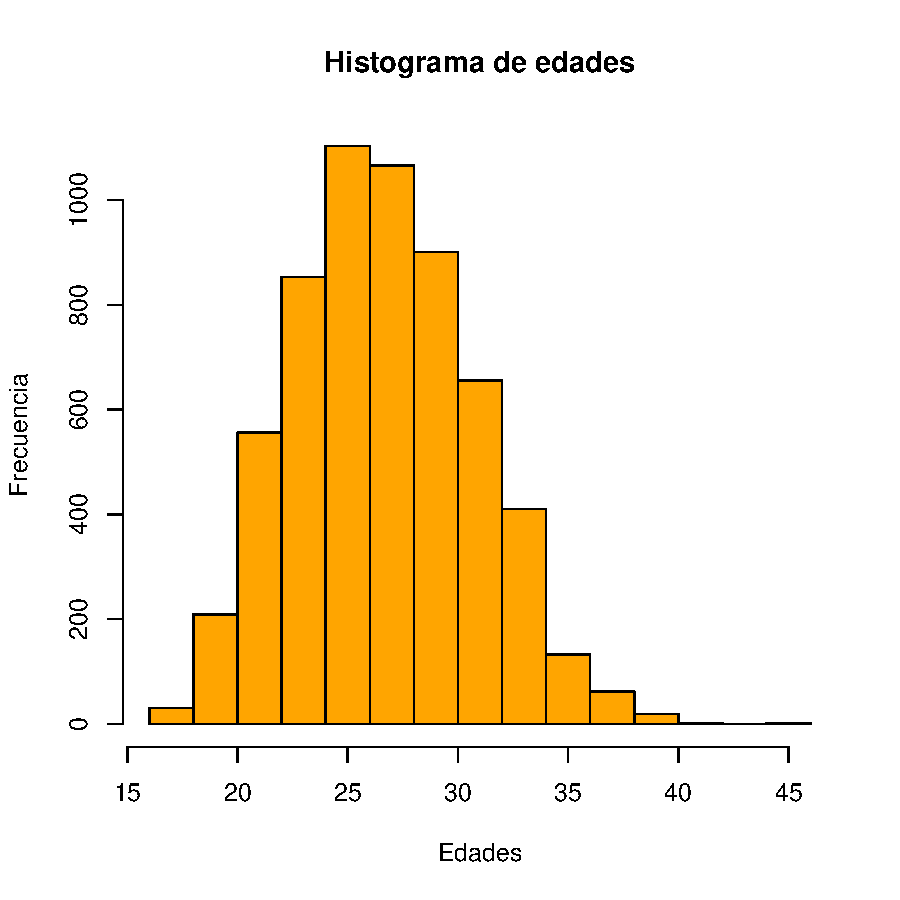
\includegraphics{Practica1-030}
\end{center}

\begin{center}
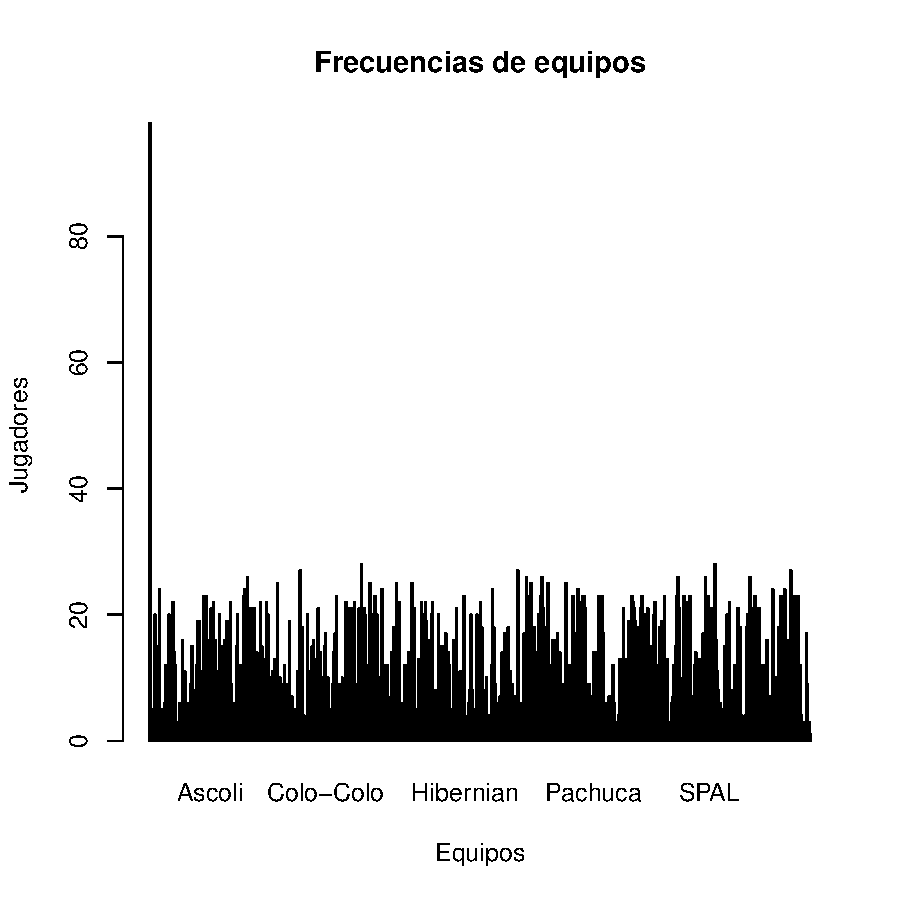
\includegraphics{Practica1-031}
\end{center}

\subsection{Medidas de centralización}
Dentro de esta sección mostraremos todas las medidas que intentan resumir los datos con un solo número, mediante la media aritmética,
la moda y la mediana.

\subsubsection{Media aritmética}
La media aritmética nos permite hacernos una idea de los valores promedios de una forma independiente, en este caso hemos calculado la media de las edades,
las medias agrupadas por equipos y nacionalidades, y la media agrupada en clases de edades. Todas ellas se han realizado con textbf{mean()}; aunque han requerido
de variaciones para las agrupaciones que se han realizado con textbf{aggregate()} en el caso de las no númericas y de textbf{cut()} junto a
 textbf{tapply()} de las númericas.
Dentro de textbf{aggregate()} se ha tenido que indicar las columnas sobre las que realizar las medias junto a la columna encargada de la 
agrupación (equipos y nacionalidades), 
además de la operación de media textbf{mean()}. Con las clases númericas ha sido necesario primero establecer el corte textbf{cut()} 
 para ello cogiendo la variable e indicando los 
cortes (breaks). Una vez definidas las clases, se ha usado textbf{tapply()} para aplicar el vector a los datos que queremos promediar, 
para ello pasando las clases, los datos y la función textbf{mean()}.

\begin{Schunk}
\begin{Sinput}
> mediaEdad <- mean(edades )
> mediaPuntos <- mean(puntuaciones )
> head(aggregate(csv[, c(2,4,5)], list(equipos), mean),20)
\end{Sinput}
\begin{Soutput}
                 Group.1      Age  Overall Potential
1                        28.16327 72.42857  74.25510
2    SSV Jahn Regensburg 29.75000 70.25000  71.00000
3  1. FC Heidenheim 1846 29.40000 71.00000  71.20000
4   1. FC Kaiserslautern 25.50000 70.00000  73.50000
5             1. FC Köln 26.15000 74.20000  77.25000
6        1. FC Magdeburg 28.00000 70.33333  70.33333
7         1. FC Nürnberg 25.28571 72.78571  76.07143
8     1. FC Union Berlin 26.73333 71.46667  74.13333
9        1. FSV Mainz 05 25.00000 73.62500  77.66667
10            Aalborg BK 24.75000 72.00000  75.75000
11             Aarhus GF 29.00000 70.00000  70.00000
12              Aberdeen 28.60000 71.80000  72.00000
13            AC Ajaccio 30.50000 70.83333  72.83333
14           AD Alcorcón 29.08333 70.33333  71.25000
15       Adelaide United 31.00000 71.50000  71.50000
16          ADO Den Haag 28.66667 71.77778  72.66667
17            AEK Athens 25.60000 72.65000  76.05000
18                   AIK 28.12500 72.12500  73.87500
19            AJ Auxerre 28.62500 71.12500  72.37500
20                  Ajax 23.27273 76.22727  81.45455
\end{Soutput}
\begin{Sinput}
> head(aggregate(csv[, c(2,4,5)], list(nacionalidades), mean),20)
\end{Sinput}
\begin{Soutput}
              Group.1      Age  Overall Potential
1             Albania 26.40000 73.10000  75.20000
2             Algeria 27.05714 74.11429  76.25714
3              Angola 26.66667 72.50000  75.50000
4           Argentina 28.35619 73.67257  75.74336
5             Armenia 27.33333 75.33333  76.33333
6           Australia 27.90625 71.93750  73.53125
7             Austria 26.29032 73.61290  76.12903
8             Belarus 30.00000 72.50000  72.50000
9             Belgium 26.43220 74.50000  77.39831
10              Benin 28.40000 72.20000  73.60000
11            Bermuda 28.00000 70.00000  70.00000
12            Bolivia 29.14286 71.00000  72.28571
13 Bosnia Herzegovina 27.25926 74.40741  76.37037
14             Brazil 27.99812 74.33898  75.95292
15           Bulgaria 29.00000 71.42857  71.85714
16       Burkina Faso 25.16667 74.16667  78.33333
17            Burundi 24.00000 71.00000  76.00000
18           Cameroon 26.94595 73.75676  76.05405
19             Canada 24.88889 72.44444  76.77778
20         Cape Verde 27.08333 74.16667  76.16667
\end{Soutput}
\begin{Sinput}
> clases <- cut(edades, breaks = c(10,20,30,40,50))
> mediaClases <- tapply(puntuaciones, list(clases ), mean)
> mediaClases 
\end{Sinput}
\begin{Soutput}
 (10,20]  (20,30]  (30,40]  (40,50] 
72.65690 73.80531 73.86630 73.00000 
\end{Soutput}
\begin{Sinput}
> mediaEquipos <- tapply(puntuaciones, list(equipos,clases ), mean)
> head(mediaEquipos ,20)
\end{Sinput}
\begin{Soutput}
                       (10,20]  (20,30]  (30,40] (40,50]
                      70.66667 72.60294 72.00000      77
 SSV Jahn Regensburg        NA 70.00000 70.50000      NA
1. FC Heidenheim 1846       NA 70.33333 72.00000      NA
1. FC Kaiserslautern        NA 70.00000       NA      NA
1. FC Köln            70.00000 74.76471 71.50000      NA
1. FC Magdeburg             NA 70.00000 71.00000      NA
1. FC Nürnberg              NA 72.78571       NA      NA
1. FC Union Berlin          NA 71.25000 72.33333      NA
1. FSV Mainz 05       69.00000 73.61905 76.00000      NA
Aalborg BK                  NA 72.00000       NA      NA
Aarhus GF                   NA 70.00000       NA      NA
Aberdeen                    NA 71.80000       NA      NA
AC Ajaccio                  NA 70.00000 71.25000      NA
AD Alcorcón                 NA 69.87500 71.25000      NA
Adelaide United             NA       NA 71.50000      NA
ADO Den Haag                NA 72.14286 70.50000      NA
AEK Athens            71.00000 72.52941 74.50000      NA
AIK                         NA 71.80000 72.66667      NA
AJ Auxerre                  NA 71.16667 71.00000      NA
Ajax                  73.12500 78.16667 77.00000      NA
\end{Soutput}
\end{Schunk}

En cuanto a la visualización de los datos se ha optado por un gráfico en el que se muestran todas las medias de las clases generado con textbf{plot()}, al 
que se le ha indicado que muestre las marcas de clases y las puntuaciones asociadas indicándose con puntos y líneas. Además, se ha añadido un punto, que representa
la media de las edades y puntuaciones con la función textbf{points()}. Finalmente se ha añadido una etiqueta al punto con la función textbf{text()}, a la que se ha tenido
que indicar además la posición para que no se superponga con el punto.

\begin{Schunk}
\begin{Sinput}
> plot(
+         seq(15, 45, by= 10),
+         mediaClases,
+         type="b",
+         col="red",
+         main="Medias",
+         xlab="Clases",
+         ylab="Puntuaciones")
> points(mediaEdad,mediaPuntos,pch=24,col="blue",bg="blue")
> text(mediaEdad,mediaPuntos, labels="Media de edad y puntuacion", cex= 0.7, pos=4)
\end{Sinput}
\end{Schunk}

\begin{center}
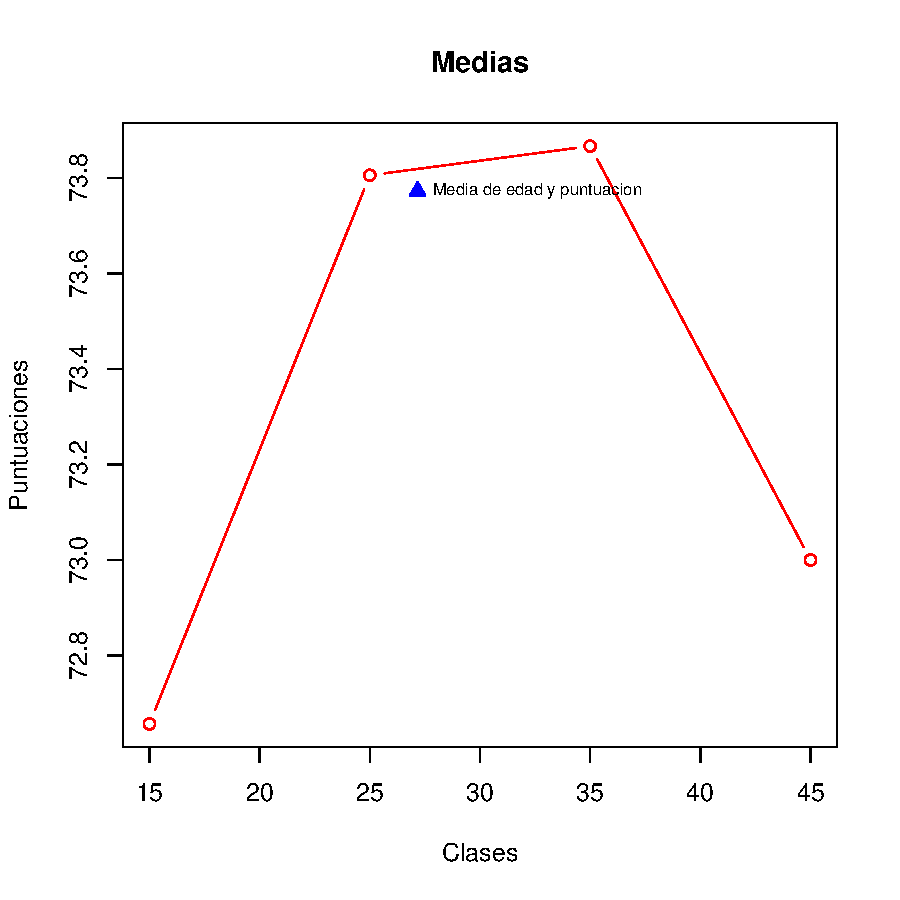
\includegraphics{Practica1-034}
\end{center}

\subsubsection{ Moda}
La moda permite saber el valor que con más frecuencia sale en la distribución de los datos, en este caso R no tenía ninguna función hecha para ello, por lo
que hemos realizado una función que lo haga. Esta función que recibe un vector por parámetro, lo primero que hace es generar 
uno quitando los duplicados contextbf{unique()}  , de tal forma
que a posteriori lo comparará con el original para contar coincidencias y devolver el mayor.

\begin{Schunk}
\begin{Sinput}
> moda <- function(v) {
+    uniqv <- unique(v)
+    uniqv[which.max(tabulate(match(v, uniqv)))]
+ }
\end{Sinput}
\end{Schunk}

Con la función ya terminada solo queda probarla sobre nuestros datos, en este caso sobre puntuaciones, nacionalidades y equipos.

\begin{Schunk}
\begin{Sinput}
> moda(puntuaciones)
\end{Sinput}
\begin{Soutput}
[1] 70
\end{Soutput}
\begin{Sinput}
> moda(nacionalidades )
\end{Sinput}
\begin{Soutput}
[1] "Spain"
\end{Soutput}
\begin{Sinput}
> moda(equipos)
\end{Sinput}
\begin{Soutput}
[1] ""
\end{Soutput}
\end{Schunk}

Como se ha podido ver equipos ha devuelto "", no se trata de un error si no que lo más frecuente de las distribución son jugadores sin equipo. Para arreglar esto
y ver cual es el equipo más representado en la muestra modificamos la variable de equipos quitando los que no tienen equipo.

\begin{Schunk}
\begin{Sinput}
> equipos<-equipos[equipos != ""]
> moda(equipos)
\end{Sinput}
\begin{Soutput}
[1] "Sporting CP"
\end{Soutput}
\end{Schunk}

\subsubsection{ Mediana}
La mediana es el valor del punto medio de un conjunto ordenado, sabiendo así la tendencia central. Para su cálculo hemos empleado el método
\textbf{median()}, que nos permite calcularla de forma directa.

\begin{Schunk}
\begin{Sinput}
> medianaEdades <- median(edades)
> medianaEdades 
\end{Sinput}
\begin{Soutput}
[1] 27
\end{Soutput}
\begin{Sinput}
> medianaPuntuaciones <- median(puntuaciones)
> medianaPuntuaciones 
\end{Sinput}
\begin{Soutput}
[1] 73
\end{Soutput}
\end{Schunk}

\subsection{Medidas de ordenación}
Las medidas de ordenación, también conocidas como medidas de posición, son los valores de la variable, que ordenados de menor a mayor, dividen a la distribución en partes.

\subsubsection{ Cuantiles}
En este caso aplicaremos diversos cuantiles, siendo la primera la división en cuartiles y la siguiente en deciles, ambas realizadas con la función que incluye \textbf{quantile()}.

\begin{Schunk}
\begin{Sinput}
> cuartiles <- quantile(puntuaciones,seq(0,1, by=0.25))
> cuartiles 
\end{Sinput}
\begin{Soutput}
  0%  25%  50%  75% 100% 
  69   71   73   76   94 
\end{Soutput}
\begin{Sinput}
> deciles<-quantile(puntuaciones, probs = seq(0, 1, by= 0.1))
> deciles
\end{Sinput}
\begin{Soutput}
  0%  10%  20%  30%  40%  50%  60%  70%  80%  90% 100% 
  69   70   70   71   72   73   74   75   76   79   94 
\end{Soutput}
\end{Schunk}

\begin{Schunk}
\begin{Sinput}
> boxplot(puntuaciones, col="orange", 
+         main = "Cuantiles de puntuaciones",
+         ylab = "Puntuaciones")
\end{Sinput}
\end{Schunk}

\begin{center}
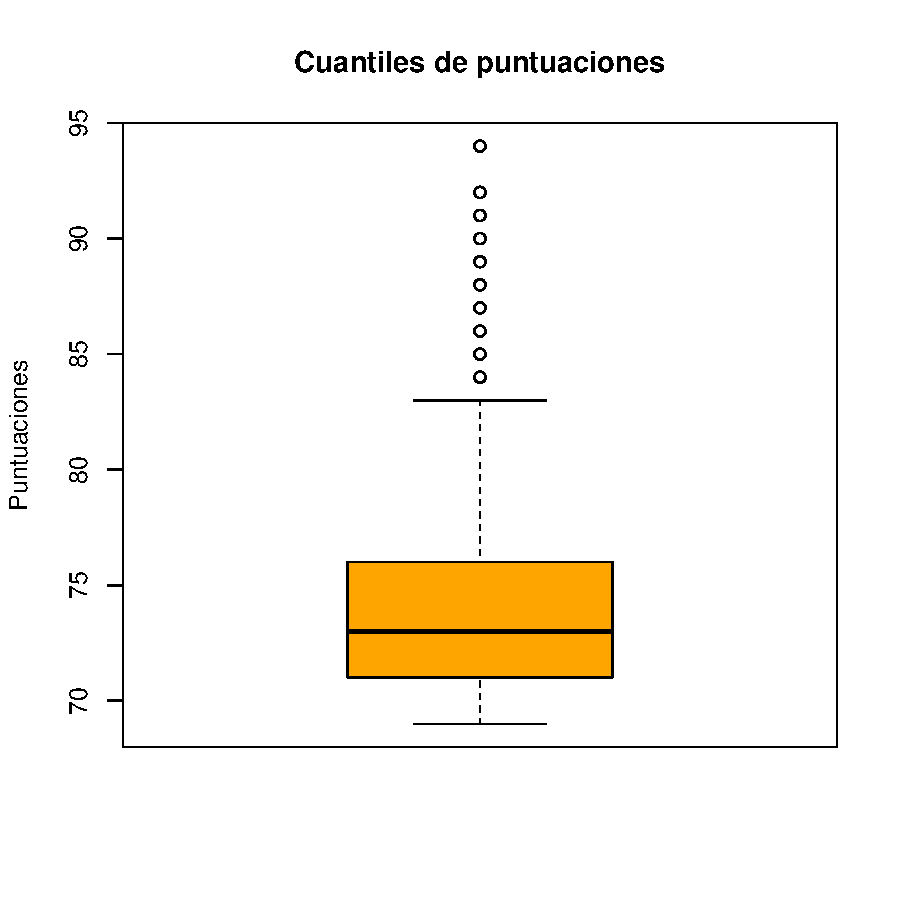
\includegraphics{Practica1-041}
\end{center}

\subsection{Medidas de dispersión}
Estas medidas sirven para mostrar la variabilidad de la distribución con respecto a las medidas de centralización. Trataremos los rangos, rangos intercuartílicos, desviaciones típicas, 
varianzas y el coeficiente variación. Además también trataremos variaciones conjuntas con la covarianza y el coeficiente de correlación.

\subsubsection{ Rango}
El rango es el valor entre el máximo y el mínimo de los datos para saber de forma sencilla la dispersión de los datos, permitiendo ver el recorrido. En este caso
como se ha explicado en el anterior ejercicio se ha tenido que hacer con las funciones \textbf{min()} y \textbf{max()}.

\begin{Schunk}
\begin{Sinput}
> rangoEdades<-(max(edades )-min(edades ))
> rangoEdades
\end{Sinput}
\begin{Soutput}
[1] 28
\end{Soutput}
\begin{Sinput}
> rangoPuntuaciones<-(max(puntuaciones )-min(puntuaciones ))
> rangoPuntuaciones
\end{Sinput}
\begin{Soutput}
[1] 25
\end{Soutput}
\end{Schunk}

\subsubsection{ Rango intercuartílico}
El rango intercuartílico a diferencia del rango, es un estadístico robusto (no se ve afectada por valores atípicos). Este consiste en calcular la diferencia entre el 
tercer cuartil y el primer cuartil, el propio R ya incluye la función \textbf{IQR()} que lo realiza sobre los datos. Se ha podido observar en el diagrama de caja que teníamos.

\begin{Schunk}
\begin{Sinput}
> rangoInterC <- IQR(edades)
> rangoInterC
\end{Sinput}
\begin{Soutput}
[1] 6
\end{Soutput}
\end{Schunk}

\subsubsection{ Desviación típica}
La desviación típica sirve para mostrar la variación entre los datos con respecto a la media aritmética. En este caso hemos empleado la función \textbf{sd()} que
la calcula directamente sobre el vector que recibe. En este caso es un valor algo alto lo que indica que produce variaciones de varias unidades con respecto a ambas medias.

\begin{Schunk}
\begin{Sinput}
> desviacionEdades <- sd(edades)
> desviacionEdades 
\end{Sinput}
\begin{Soutput}
[1] 4.077593
\end{Soutput}
\begin{Sinput}
> desviacionPuntos <- sd(puntuaciones)
> desviacionPuntos 
\end{Sinput}
\begin{Soutput}
[1] 3.884298
\end{Soutput}
\begin{Sinput}
> head(aggregate(csv[, c(2,4,5)], list(nacionalidades), sd),20)
\end{Sinput}
\begin{Soutput}
              Group.1      Age  Overall Potential
1             Albania 2.503331 4.254409  5.940445
2             Algeria 3.621365 4.247985  4.742442
3              Angola 4.926121 3.016621  4.183300
4           Argentina 4.463116 3.682384  4.436352
5             Armenia 2.081666 6.806859  5.773503
6           Australia 3.559262 2.340906  3.162118
7             Austria 3.489502 3.245955  4.240646
8             Belarus 1.414214 3.535534  3.535534
9             Belgium 4.209226 5.113665  5.438294
10              Benin 3.286335 2.167948  4.929503
11            Bermuda       NA       NA        NA
12            Bolivia 5.145502 1.825742  3.251373
13 Bosnia Herzegovina 3.380858 4.439848  3.962790
14             Brazil 4.011540 4.121958  4.964368
15           Bulgaria 2.581989 2.572751  3.236694
16       Burkina Faso 4.167333 2.401388  4.273952
17            Burundi       NA       NA        NA
18           Cameroon 3.681379 3.103810  3.807492
19             Canada 3.982601 1.878238  4.737557
20         Cape Verde 3.369875 3.128559  4.608950
\end{Soutput}
\end{Schunk}

\subsubsection{ Varianza}
La varianza permite al igual que la desviación típica calcular las variaciones de los datos, aunque con las unidades al cuadrado. En este caso se
hará directamente con la función \textbf{var()}. Al igual que antes los datos arrojados permiten ver que las variaciones son significantes.

\begin{Schunk}
\begin{Sinput}
> varianzaEdades <- var(edades)
> varianzaEdades 
\end{Sinput}
\begin{Soutput}
[1] 16.62677
\end{Soutput}
\begin{Sinput}
> var(puntuaciones)
\end{Sinput}
\begin{Soutput}
[1] 15.08777
\end{Soutput}
\end{Schunk}

\subsubsection{ Coeficiente de variación}
El coeficiente de variación es la relación entre la media y la variabilidad de la variable. Para calcularlo solo hace falta dividir la desviación típica con respecto a su media, en este
caso es baja lo que indica que a pesar de que parezca que hay bastante desviación típica, no lo es con respecto a la media.

\begin{Schunk}
\begin{Sinput}
> coefVariacion <- desviacionEdades/mediaEdad
> coefVariacion
\end{Sinput}
\begin{Soutput}
[1] 0.1500835
\end{Soutput}
\end{Schunk}

\subsubsection{ Covarianza}
La covarianza es un valor que nos indical a variación conjunta de dos variables con respecto a sus medias, permitiendo saber si existe una dependencia entre ambas variables.
Se aplica en R mediante la función \textbf{cov()} que se encarga de realizar la covarianza entre las dos variables que reciba. En nuestros datos la covarianza tiene un valor muy bajo lo
que indica que la dependencia entre las variables de edades y puntuaciones es muy baja.

\begin{Schunk}
\begin{Sinput}
> covarianza<-cov(edades, puntuaciones)  
> covarianza
\end{Sinput}
\begin{Soutput}
[1] 0.5882306
\end{Soutput}
\end{Schunk}

\subsubsection{ Coeficiente de correlación}
La correlación indica la fuerza dirección de una relación lineal entre dos variables variando entre -1 y 1. Según estos valores se acerquen a los extremos tendrán mayor fuerza pudiendo ser negativa
o positiva si son lineales o inversas las relaciones, si se acerca al 0 no hay relación alguna. En nuestro caso tiene un valor muy próximo a 0 por lo que no hay relación alguna entre ambas.

\begin{Schunk}
\begin{Sinput}
> cor(edades, puntuaciones)
\end{Sinput}
\begin{Soutput}
[1] 0.03713908
\end{Soutput}
\end{Schunk}


\end{document}
